\section{Introducción}

\subsection{Evolución de la Concurrencia en Java}
\begin{frame}
    \begin{center}
        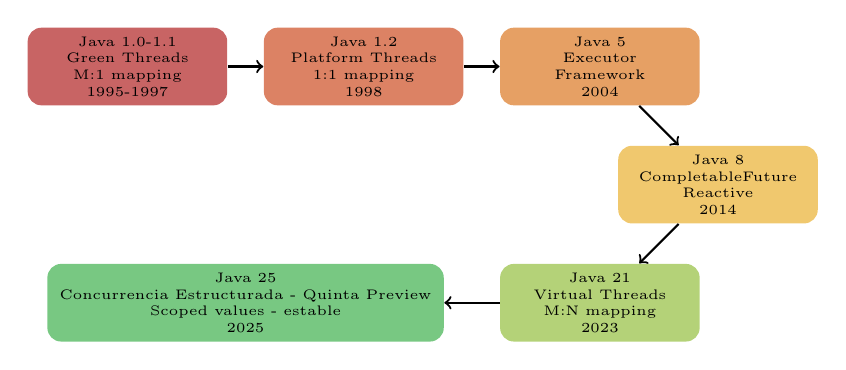
\begin{tikzpicture}[
            box/.style={rectangle, text width=2.3cm, align=center,
            font=\tiny, rounded corners=5pt},
            box1/.style={box, fill={rgb,255: red,200; green,100; blue,100}},
            box2/.style={box, fill={rgb,255: red,220; green,130; blue,100}},
            box3/.style={box, fill={rgb,255: red,230; green,160; blue,100}},
            box4/.style={box, fill={rgb,255: red,240; green,200; blue,110}},
            box5/.style={box, fill={rgb,255: red,180; green,210; blue,120}},
            box6/.style={box, text width=4.8cm, fill={rgb,255: red,120; green,200; blue,130}}
        ]
            \node (green) [box1] at (-4.5, 1.5) {Java 1.0-1.1\\Green Threads\\M:1 mapping\\1995-1997};
            \node (platform) [box2] at (-1.5, 1.5) {Java 1.2\\Platform Threads\\1:1 mapping\\1998};
            \node (executor) [box3] at (1.5, 1.5) {Java 5\\Executor\\Framework\\2004};
            \node (reactive) [box4] at (3, 0) {Java 8\\CompletableFuture\\Reactive\\2014};
            \node (virtual) [box5] at (1.5, -1.5) {Java 21\\Virtual Threads\\M:N mapping\\2023};
            \node (structured) [box6] at (-3, -1.5) {Java 25\\Concurrencia Estructurada - Quinta Preview\\Scoped values - estable \\2025};

            \draw [->, thick] (green) -- (platform);
            \draw [->, thick] (platform) -- (executor);
            \draw [->, thick] (executor) -- (reactive);
            \draw [->, thick] (reactive) -- (virtual);
            \draw [->, thick] (virtual) -- (structured);
        \end{tikzpicture}
    \end{center}
    \begin{alertblock}{Estado en Java 25}
        \begin{itemize}
            \item Virtual Threads: \textbf{Estable} (desde Java 21)
            \item Scoped Values: \textbf{Estable} desde Java 25 ~\cite{JEP506}
            \item Concurrencia Estructurada: \textbf{Quinta Preview} en Java 25 ~\cite{JEP505}
        \end{itemize}
    \end{alertblock}
\end{frame}

\subsection{Programación estructurada}
\begin{frame}
    \frametitle{¡La promesa!}
    \begin{itemize}[<+->]
    \item Código que \textbf{se lee como se ejecuta}
    \item Rendimiento equiparable a programación reactiva, con beneficios.
    \item Sin callbacks.
    \item \textbf{De vuelta a la simplicidad}
    \end{itemize}
\end{frame}

\subsection{Problema de ejemplo: Procesamiento de Transacción Financiera}
\begin{frame}
    \frametitle{Flujo ficticio}
    \begin{center}

        \begin{tikzpicture}[
            node/.style={rectangle, rounded corners, text width=2cm, align=center, font=\tiny, minimum height=0.8cm, draw=none},
            parallel/.style={rectangle, rounded corners, text width=2.8cm, align=center, font=\tiny, fill=blue!10, minimum height=0.8cm, draw=none},
            arrow/.style={->, thick, rounded corners}
        ]

% Nodes positioned horizontally (left to right)
            \node (transaction) [node, fill=purple!20] at (0,0) {Transacción (input)};

% First parallel: Merchant and Consumer paths
            \node (merchant) [node, fill=green!20] at (5,1) {Validar Comercio \\ 500ms };
            \node (card) [node, fill=green!20] at (3,-1) {Validar Tarjeta \\ 100ms};

% Parallel validations - perfectly aligned vertically
            \node (balance) [parallel] at (6.5,0) {Validar Saldo \\ 600ms};
            \node (pin) [parallel] at (6.5,-1) {Validar PIN \\ 300ms};
            \node (expiry) [parallel] at (6.5,-2) {Validar Expiración \\ 200ms};

            \node (transfer) [node, fill=orange!20] at (10,-0.5) {Transferir \\ Monto };

% Coordination points for line division and convergence
            \coordinate (split1) at (1.5,0);
            \coordinate (split2) at (4.5,-1);
            \coordinate (join) at (8.5,-0.5);

% Arrows with structured lines
% From transaction to first split
            \draw [thick] (transaction.east) -- (split1);

% From split1 to merchant and card paths
            \draw [arrow] (split1) -- (1.5,1) -- (merchant.west);
            \draw [arrow] (split1) -- (1.5,-1) -- (card.west);

% From card to split2 for parallel validations
            \draw [thick] (card.east) -- (split2);

% From split2 to parallel validations (vertical then horizontal)
            \draw [arrow] (split2) -- (4.5,0) -- (balance.west);
            \draw [arrow] (split2) -- (pin.west);
            \draw [arrow] (split2) -- (4.5,-2) -- (expiry.west);

% From merchant to join point
            \draw [--, thick, rounded corners] (merchant.east) -- (8.5,1) -- (join);

% From parallel validations to join point (horizontal then vertical)
            \draw [--, thick, rounded corners] (balance.east) -- (8.5,0) -- (join);
            \draw [--, thick, rounded corners] (pin.east) -- (8.5,-1) -- (join);
            \draw [--, thick, rounded corners] (expiry.east) -- (8.5,-2) -- (join);

% From join point to transfer
            \draw [arrow] (join) -- (transfer.west);

% Labels
            \node at (1.5,1.5) [font=\tiny]{\textbf{En Paralelo: comercio y consumidor}};
            \node at (4.5,-2.6) [font=\tiny] {\textbf{En Paralelo: propiedades de la tarjeta}};

        \end{tikzpicture}
    \end{center}

    \begin{exampleblock}{Flujo Optimizado}
        \textbf{1.} En paralelo: validar comercio y consumidor (tarjeta)\\
        \textbf{2.} Validaciones paralelas de tarjeta (saldo, PIN, expiración)\\
        \textbf{3.} Transferir sólo si todas las validaciones pasan
    \end{exampleblock}
\end{frame}

%\subsection{Demo Setup: Quarkus REST API}
%\begin{frame}[fragile]
%    \begin{block}{Iniciando la aplicación}
%        \begin{minted}[fontsize=\footnotesize]{bash}
%./gradlew quarkusDev
%        \end{minted}
%    \end{block}
%
%    \vspace{1em}
%
%    \begin{block}{Verificando que funciona}
%        \begin{minted}[fontsize=\footnotesize]{bash}
%curl http://localhost:8080/api/health
%        \end{minted}
%    \end{block}
%
%    \vspace{1em}
%
%    \begin{exampleblock}{Endpoints disponibles}
%        \begin{itemize}
%            \item \texttt{POST /api/reactive/basic} - CompletableFuture básico
%            \item \texttt{POST /api/reactive/fail-fast} - Reactive con fail-fast manual
%            \item \texttt{POST /api/structured/normal} - Structured Concurrency (await all)
%            \item \texttt{POST /api/structured/fail-fast} - Structured con fail-fast automático
%            \item \texttt{POST /api/compare} - Comparación de performance
%        \end{itemize}
%    \end{exampleblock}
%\end{frame}
